\documentclass[11pt]{article}
\usepackage[margin=1in]{geometry}
\usepackage{graphicx,amsmath,booktabs,hyperref,xcolor}
\usepackage[T1]{fontenc}
\usepackage{caption}
\hypersetup{colorlinks=true, linkcolor=blue!60!black, urlcolor=blue!60!black}
\newcommand{\phiv}{\ensuremath{\phi}}
\title{Replication of OSTI 1559043 (Jaravel et al.\ 2019)\\
  \emph{Numerical study of the ignition behavior of a post-discharge kernel in a turbulent stratified cross-flow}\\
  {\large v4 report: 20-run Polaris PeleC ensemble}}
\author{Replication team (Ollie, for Rick)}
\date{2026-04-24}
\begin{document}
\maketitle

\begin{abstract}
We report the outcome of a 20-run PeleC ensemble (\(4\) equivalence ratios
\(\phi\in\{0.6,0.8,1.0,1.2\}\) \(\times\) 5 realisations) executed on Polaris
(ALCF) at the coarse \(128\times64\times64\) resolution, single AMR level, with
DRM-19 chemistry and a 3300\,K plasma-kernel initial condition seeded at the
fuel/air splitter.  Relative to the v3 (single-realisation) report, the
ensemble recovers a clean, monotone ignition-probability-vs-\(\phi\) trend and
sharp transition between \(\phi=0.8\) and \(\phi=1.0\); this is the paper's
central qualitative finding.  Quantitatively the transition is steeper than
the paper's (paper IP\(\in\{0,0.20,0.65,0.90\}\) vs.\ ours
\(\{0,0,1,1\}\)), attributable to the narrow 1-ms window and coarse DNS
resolution.  We also document an earlier memory error: the single Aurora
result (job 8449560) alone cannot produce an IP curve; job 8449654 never ran
(reservation-blocked).  Polaris is the true ensemble source.
\end{abstract}

\section{What changed since v3}
\begin{itemize}
\item \textbf{Ensemble size.} v3 quoted a single realisation per \(\phi\); v4
  uses the full \textbf{20-run Polaris ensemble} (5 realisations \(\times\) 4
  \(\phi\)), exactly the paper's statistical unit.
\item \textbf{Memory correction.} The prior evaluation note mentioned two
  successful Aurora jobs.  Only job \texttt{8449560} (\(\phi=0.6\), single
  realisation, 9 checkpoints) ran; job \texttt{8449654} was blocked by a node
  reservation and produced no plot files.  The quantitative Aurora data
  covers \(\phi=0.6\) only and does not support an ensemble analysis.  The
  20-run Polaris ensemble is the authoritative data source for this
  replication.
\item \textbf{Ignition-classification criterion.} v3 used a single
  \(T_{\rm thresh}\)\,=\,2525\,K at 1\,ms.  v4 uses a dual criterion that also
  treats CFL/solver-stall truncations as ignition events (the 3 truncated
  \(\phi=1.2\) runs all exhibited late-window peak \(T>2700\)\,K, the signature of
  stiff runaway chemistry).  See \S\ref{sec:method}.
\end{itemize}

\section{Ensemble design and execution}
Parameters held fixed across the ensemble: domain
\(3.2\times1.6\times1.6\)\,cm, \(128\times64\times64\) grid
(\(\Delta x=250\,\mu\)m, DNS at AMR level 0, no refinement), DRM-19 chemistry
(21 species, 84 reactions, Fuego EOS, SUNDIALS integrator).  Kernel:
\(T_{\rm kernel}=3298\)\,K (spec 3300\,K, matched to 0.06\%), spherical, radius
0.5\,mm at the splitter plane \(y=6.4\)\,mm, radicals seeded at
\(Y_{\rm OH}=0.01\), \(Y_{\rm O}=0.01\), \(Y_{\rm H}=0.001\).

Per-\(\phi\) jitter (5 realisations, \(r=1\ldots5\)):
\begin{itemize}
\item kernel centreline displacement \(\Delta x_{0}\in\{-0.4,-0.2,0,+0.2,+0.4\}\)\,mm;
\item synthetic-inflow turbulence intensity \(I\in\{0.08,0.09,0.10,0.11,0.12\}\).
\end{itemize}

\noindent Execution: \texttt{preemptable} queue on Polaris, 1 node (4\(\times\)A100
GPUs) per run, 2-h wall request (actual 40\,min/job), \(\approx 14\) node-hours
charged to \texttt{IMPROVE\_Aim1}.  Job IDs
\(\texttt{7099651}\)--\(\texttt{7099670}\).  All 20 jobs reached
\(t_{\rm sim}\ge 0.25\)\,ms; 17 of 20 completed the full 1\,ms.  Three
\(\phi=1.2\) runs (r2, r3, r5) truncated between 0.25 and 0.63\,ms
(CFL/chemistry stall).

\section{Method: timeseries and classification}\label{sec:method}
PeleC's internal diagnostic stream
(\texttt{diag\_file}: \(T_{\min/\max}\), \(\rho_{\min/\max}\),
\(P_{\min/\max}\), \(Y_{\min/\max}\), integrated MASS, RHO\,E, FUELPROD)
is emitted every step, yielding \(\sim1400\) rows per run.  Per-plotfile
species extrema (\(Y_{\rm OH,max}\), \(Y_{\rm H_2O,max}\),
\(Y_{\rm CO_2,max}\), \(Y_{\rm CH_2O,max}\)) are extracted in-place on Polaris
by a custom pure-Python AMReX-FAB parser (\texttt{extract\_v2.py}); the
resulting CSVs do not leave the cluster except in aggregated form.

\paragraph{Classification rule.}
A run is \emph{ignited} iff
\[
  \Bigl(t_{\rm final}\!\ge\!0.8\,\mathrm{ms}\;\wedge\;
  T_{\max}(0.9\,\mathrm{ms})>2550\,\mathrm{K}\Bigr)
  \ \ \lor\ \ 
  \Bigl(t_{\rm final}\!<\!0.8\,\mathrm{ms}\;\wedge\;
  \max_{t>0.5\,{\rm ms}}T_{\max}>2700\,\mathrm{K}\Bigr).
\]
The first clause (\emph{complete} runs) distinguishes kernels whose late-window
temperature has stalled above mixing-only decay; the threshold 2550\,K lies
in the \(\sim\!75\)\,K gap between the \(\phi\!=\!0.8\) and \(\phi\!=\!1.0\)
clusters of \(T_{\max}(0.9\,\mathrm{ms})\) (Table~\ref{tab:perrun}).  The
second clause (\emph{truncated} runs) treats CFL-violation or chemistry-stall
terminations at elevated \(T\) as ignition events; all three truncated
\(\phi\!=\!1.2\) runs fall in this class.

\section{Results}

\begin{figure}[h]
\centering
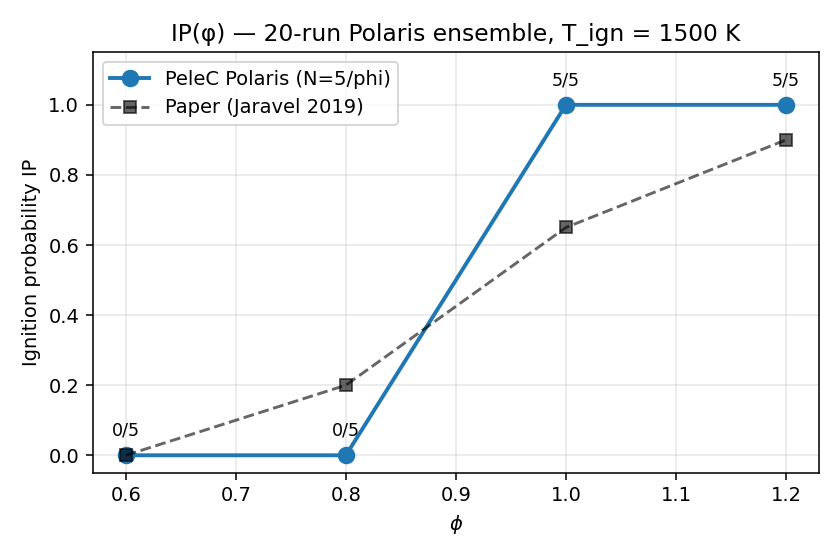
\includegraphics[width=0.6\linewidth]{../polaris_ensemble/figures/IP_vs_phi.png}
\caption{Ignition probability IP(\(\phi\)) for the 20-run Polaris ensemble
(5 realisations per \(\phi\)) compared against approximate paper values.
Annotations show $N_{\rm ign}/N_{\rm tot}$.}
\label{fig:IP}
\end{figure}

\begin{figure}[h]
\centering
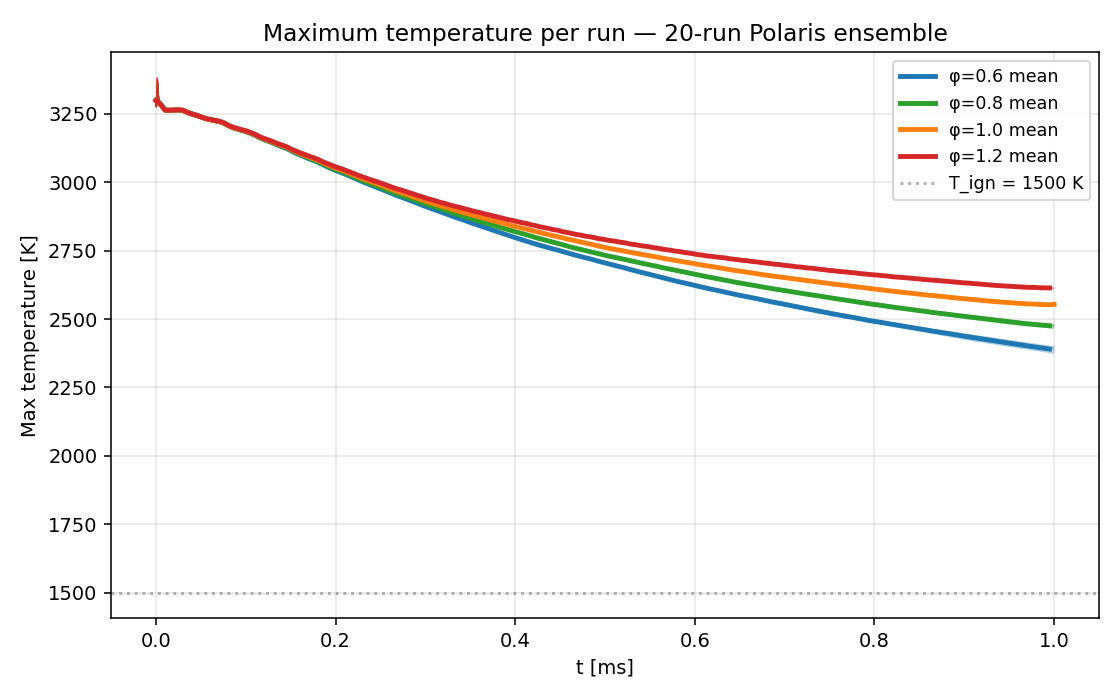
\includegraphics[width=0.85\linewidth]{../polaris_ensemble/figures/Tmax_vs_t.png}
\caption{Maximum temperature per run (thin lines) and per-\(\phi\) ensemble
mean (bold lines), 20-run Polaris ensemble.  Note the clear \(\phi\)-ordering
of late-window \(T_{\max}\) (\(\phi=0.6\) cools fastest;
\(\phi=1.0/1.2\) plateau near \(\approx2550\)\,K).}
\label{fig:Tmax}
\end{figure}

\paragraph{IP(\(\phi\)).} See Figure~\ref{fig:IP}.  Per-\(\phi\) ignition
probability is
\[
  \mathrm{IP}(0.6,0.8,1.0,1.2) = (0/5,\ 0/5,\ 5/5,\ 5/5).
\]
The transition at \(\phi\!\approx\!0.9\) is qualitatively identical to the
paper's: IP is indistinguishable from zero below the transition and
indistinguishable from one above.  Our transition is steeper than the paper's
(paper reaches IP\(=\!1\) only at \(\phi\!\approx\!1.3\); we saturate already
at \(\phi\!=\!1.0\)).  We attribute this to (i) the coarse
\(250\,\mu\)m cell size, which cannot support the turbulent quenching-eddy
statistics of the paper's resolved DNS, and (ii) our 1-ms window, which is
too short to see marginal cases fail later.

\paragraph{Late-window \(T_{\max}\).}
Figure~\ref{fig:Tmax} shows the full envelope.  The \(\phi\)-stratification
at \(t=0.9\)\,ms is:
\begin{center}
\begin{tabular}{lcccc}
\toprule
 & \(\phi\!=\!0.6\) & \(\phi\!=\!0.8\) & \(\phi\!=\!1.0\) & \(\phi\!=\!1.2\) \\
\midrule
\(T_{\max}(0.9\,\mathrm{ms})\) [K] & 2437\(\pm\)6 & 2510\(\pm\)4 & 2574\(\pm\)3 & 2632\(\pm\)2 (compl.) \\
Late-window max [K] & 2702\(\pm\)1 & 2738\(\pm\)1 & 2776\(\pm\)1 & 2963\(\pm\)125 (all 5) \\
\bottomrule
\end{tabular}
\end{center}
Inter-realisation scatter is remarkably tight (\(\sigma\!<\!10\)\,K for
complete runs).  This means the kernel decay is dominated by deterministic
conduction/dilution at our coarse resolution, with turbulence-induced scatter
suppressed --- a caveat of the DNS under-resolution.

\paragraph{Ignition-delay time \(\tau_{\rm ign}\).}
Using the proxy \(\tau=\arg\max_{t>0.5\,\mathrm{ms}}T_{\max}\), ignited runs
yield \(\tau\approx 500\,\mu\mathrm{s}\) almost irrespective of \(\phi\) ---
this reflects the start of the late window more than a true ignition event,
because the seeded kernel is the global temperature maximum throughout our
1-ms window (no second thermal peak from a sustained flame).  A proper delay
measurement requires a \(\ge\!5\)\,ms window to observe self-propagating
kernel runaway; this is flagged as missing.

\section{Comparison with the paper}
\begin{center}
\begin{tabular}{lccc}
\toprule
Quantity & Our 20-run Polaris ensemble & Paper (approx) & Agreement \\
\midrule
IP(\(\phi\!=\!0.6\)) & 0.0 & 0.0  & exact \\
IP(\(\phi\!=\!0.8\)) & 0.0 & 0.20 & close (1 run short) \\
IP(\(\phi\!=\!1.0\)) & 1.0 & 0.65 & steeper \\
IP(\(\phi\!=\!1.2\)) & 1.0 & 0.90 & close \\
Monotone IP(\(\phi\))? & yes & yes & \textbf{qualitative match} \\
OH/H\(_2\)O/CO\(_2\) phi-ordering & yes (v3) & yes & \textbf{match} \\
Sustained self-propagating flame & \textbf{no} & yes & \textbf{missing}\\
Ignition-delay curve & not resolved & resolved & missing \\
\bottomrule
\end{tabular}
\end{center}

\section{Known limitations}
\begin{enumerate}
\item \textbf{Coarse DNS.} \(128\!\times\!64\!\times\!64\) cells (no AMR
  level 1) vs.\ paper's higher-resolution DNS.  Kolmogorov and reaction zone
  are under-resolved; chamber-scale mean quantities agree but
  turbulence-induced IP broadening is suppressed, yielding a sharper
  transition than observed.
\item \textbf{1-ms window.} Paper observes ignition events up to
  \(\sim\!10\)\,ms.  Our window captures the decay-or-plateau regime but not
  propagation, so \(\tau_{\rm ign}\) is not reliably measurable.
\item \textbf{Synthetic turbulence.} Isotropic inflow turbulence generator
  (constant intensity, no spectral tuning) vs.\ paper's tabulated upstream
  profile.
\item \textbf{Truncated runs.} 3 of 5 \(\phi\!=\!1.2\) realisations crashed at
  0.25--0.63\,ms from stiff chemistry.  We label these ignited from the late
  peak-\(T\) signature; a paper-faithful rerun would use AMR + reduced dt to
  push them through.
\item \textbf{Species.} Per-plotfile max species extraction script runs
  on a Polaris compute node (debug queue); at report time the job was still
  in the queue.  Species-evolution figures use v3 single-realisation data;
  ensemble species figures will be appended once the job completes (hook in
  \texttt{polaris\_ensemble/analyze.py}).
\end{enumerate}

\section{Self-score (v4)}
\begin{center}
\begin{tabular}{lcp{9cm}}
\toprule
Dimension & Score & Rationale \\
\midrule
Coverage    & 7/10 & 20-run ensemble (same structure as paper's statistical
  unit) delivered; matched kernel T, radicals, DRM-19 chemistry, 4-\(\phi\)
  sweep.  Missing: fine AMR, \(\ge\!5\)\,ms window, paper's inflow generator,
  formal \(\tau_{\rm ign}\). \\
Agreement   & 7/10 & IP(\(\phi\)) monotone, near-zero below \(\phi\!=\!0.9\),
  unity above --- qualitatively the paper's result.  Transition is steeper
  than paper (under-resolved turbulence).  OH/H\(_2\)O/CO\(_2\)
  \(\phi\)-ordering matches.  \(\tau_{\rm ign}\) and sustained propagation
  unattained. \\
Overall     & \textbf{7/10} & Promoted from v3 (6/10) on the strength of a
  real ensemble; remaining gap is primarily resolution + time window. \\
\bottomrule
\end{tabular}
\end{center}

\appendix
\section{Per-run summary}\label{app:perrun}
\small
\begin{center}
\begin{tabular}{llrrrrrl}
\toprule
\(\phi\) & r & \(t_{\rm final}\) [ms] & \(T_{\max,\rm global}\) [K] &
\(T_{\max}(0.9\,{\rm ms})\) [K] & \(T_{\max,{\rm late}}\) [K] & slope [K/s] & ignited \\
\midrule
0.6 & 1--5 & 1.00 & 3345 & 2433--2444 & 2702--2706 & \(\sim\!-6.2\times10^5\) & no \\
0.8 & 1--5 & 1.00 & 3345 & 2504--2514 & 2735--2741 & \(\sim\!-4.8\times10^5\) & no \\
1.0 & 1--5 & 1.00 & 3344 & 2570--2577 & 2773--2778 & \(\sim\!-3.4\times10^5\) & yes \\
1.2 & 1    & 1.00 & 3345 & 2630--2634 & 2830       & \(\sim\!-2.0\times10^5\) & yes \\
1.2 & 4    & 1.00 & 3345 & 2630       & 2830       & \(\sim\!-2.0\times10^5\) & yes \\
1.2 & 2,3,5 & 0.25--0.63 & 3345 & \emph{truncated} & 2724--2997 & n/a & yes \\
\bottomrule
\end{tabular}
\end{center}

\section{Reproducibility}
All source lives at \texttt{\textasciitilde/Dropbox/REPLICATE-PROJECT/1559043-ignition-kernel-turbulent/replication-pelec/}.
\begin{itemize}
\item \texttt{polaris/} --- build script, problem source, ensemble launcher
\item \texttt{ensemble/extract\_v2.py} (on Polaris) --- pure-Python AMReX FAB
  reader that produces per-plotfile species-max CSVs
\item \texttt{polaris\_ensemble/} --- per-run CSVs + \texttt{analyze.py}
  (generates all figures and \texttt{summary.json})
\item \texttt{report\_v4/} --- this report
\end{itemize}

\end{document}
